% !TEX root = ../SANER2027-main-labeling.tex
% Approach
% kNN voting baseline, RAG, filtered RAG (with its calibration), LoRA fine-tuning baseline

\section{Approach}
\label{sec:03_approach}

\begin{comment}
\begin{figure}[t]
    \centering
    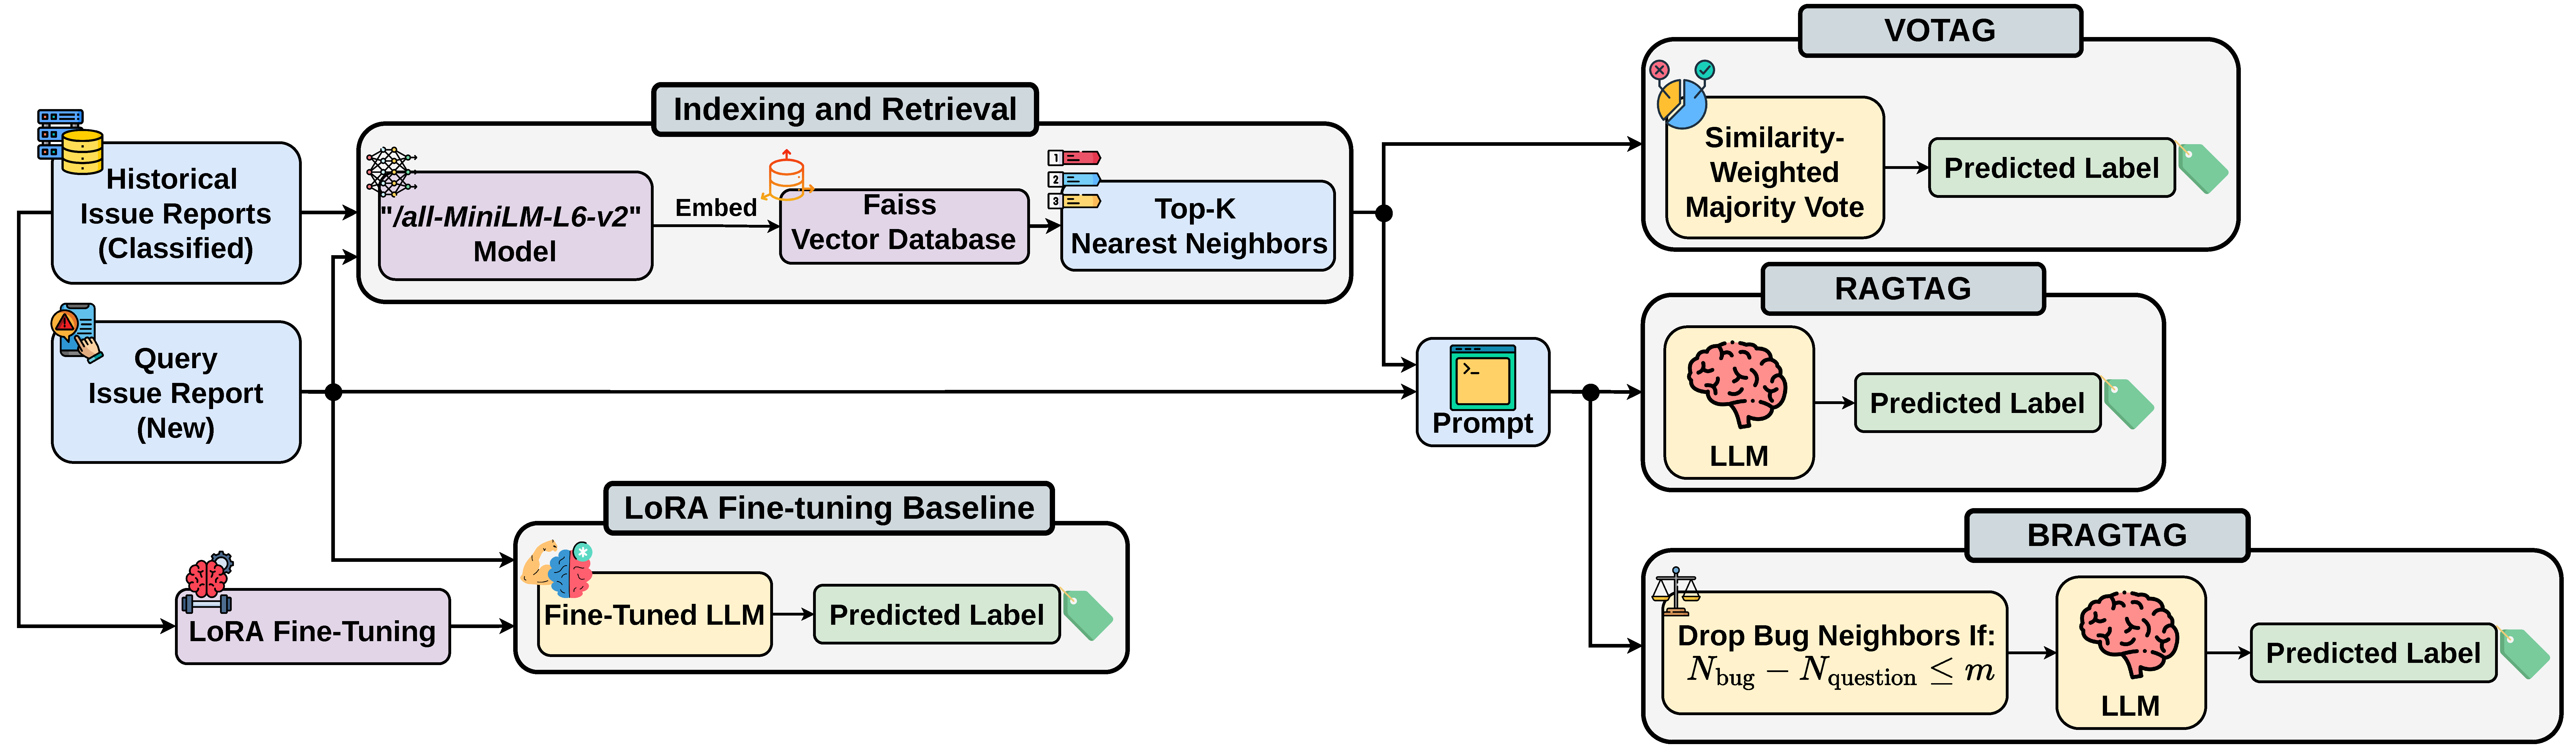
\includegraphics[width=\linewidth]{figures/app_ov.pdf}
    \caption{Overview of the $k$NN voting baseline, retrieval-augmented few-shot prompting (RAG), filtered RAG, and the LoRA fine-tuning baseline.}
    \label{fig:approach-overview}
\end{figure}
\end{comment}

\begin{figure*}[!t]
    \centering
    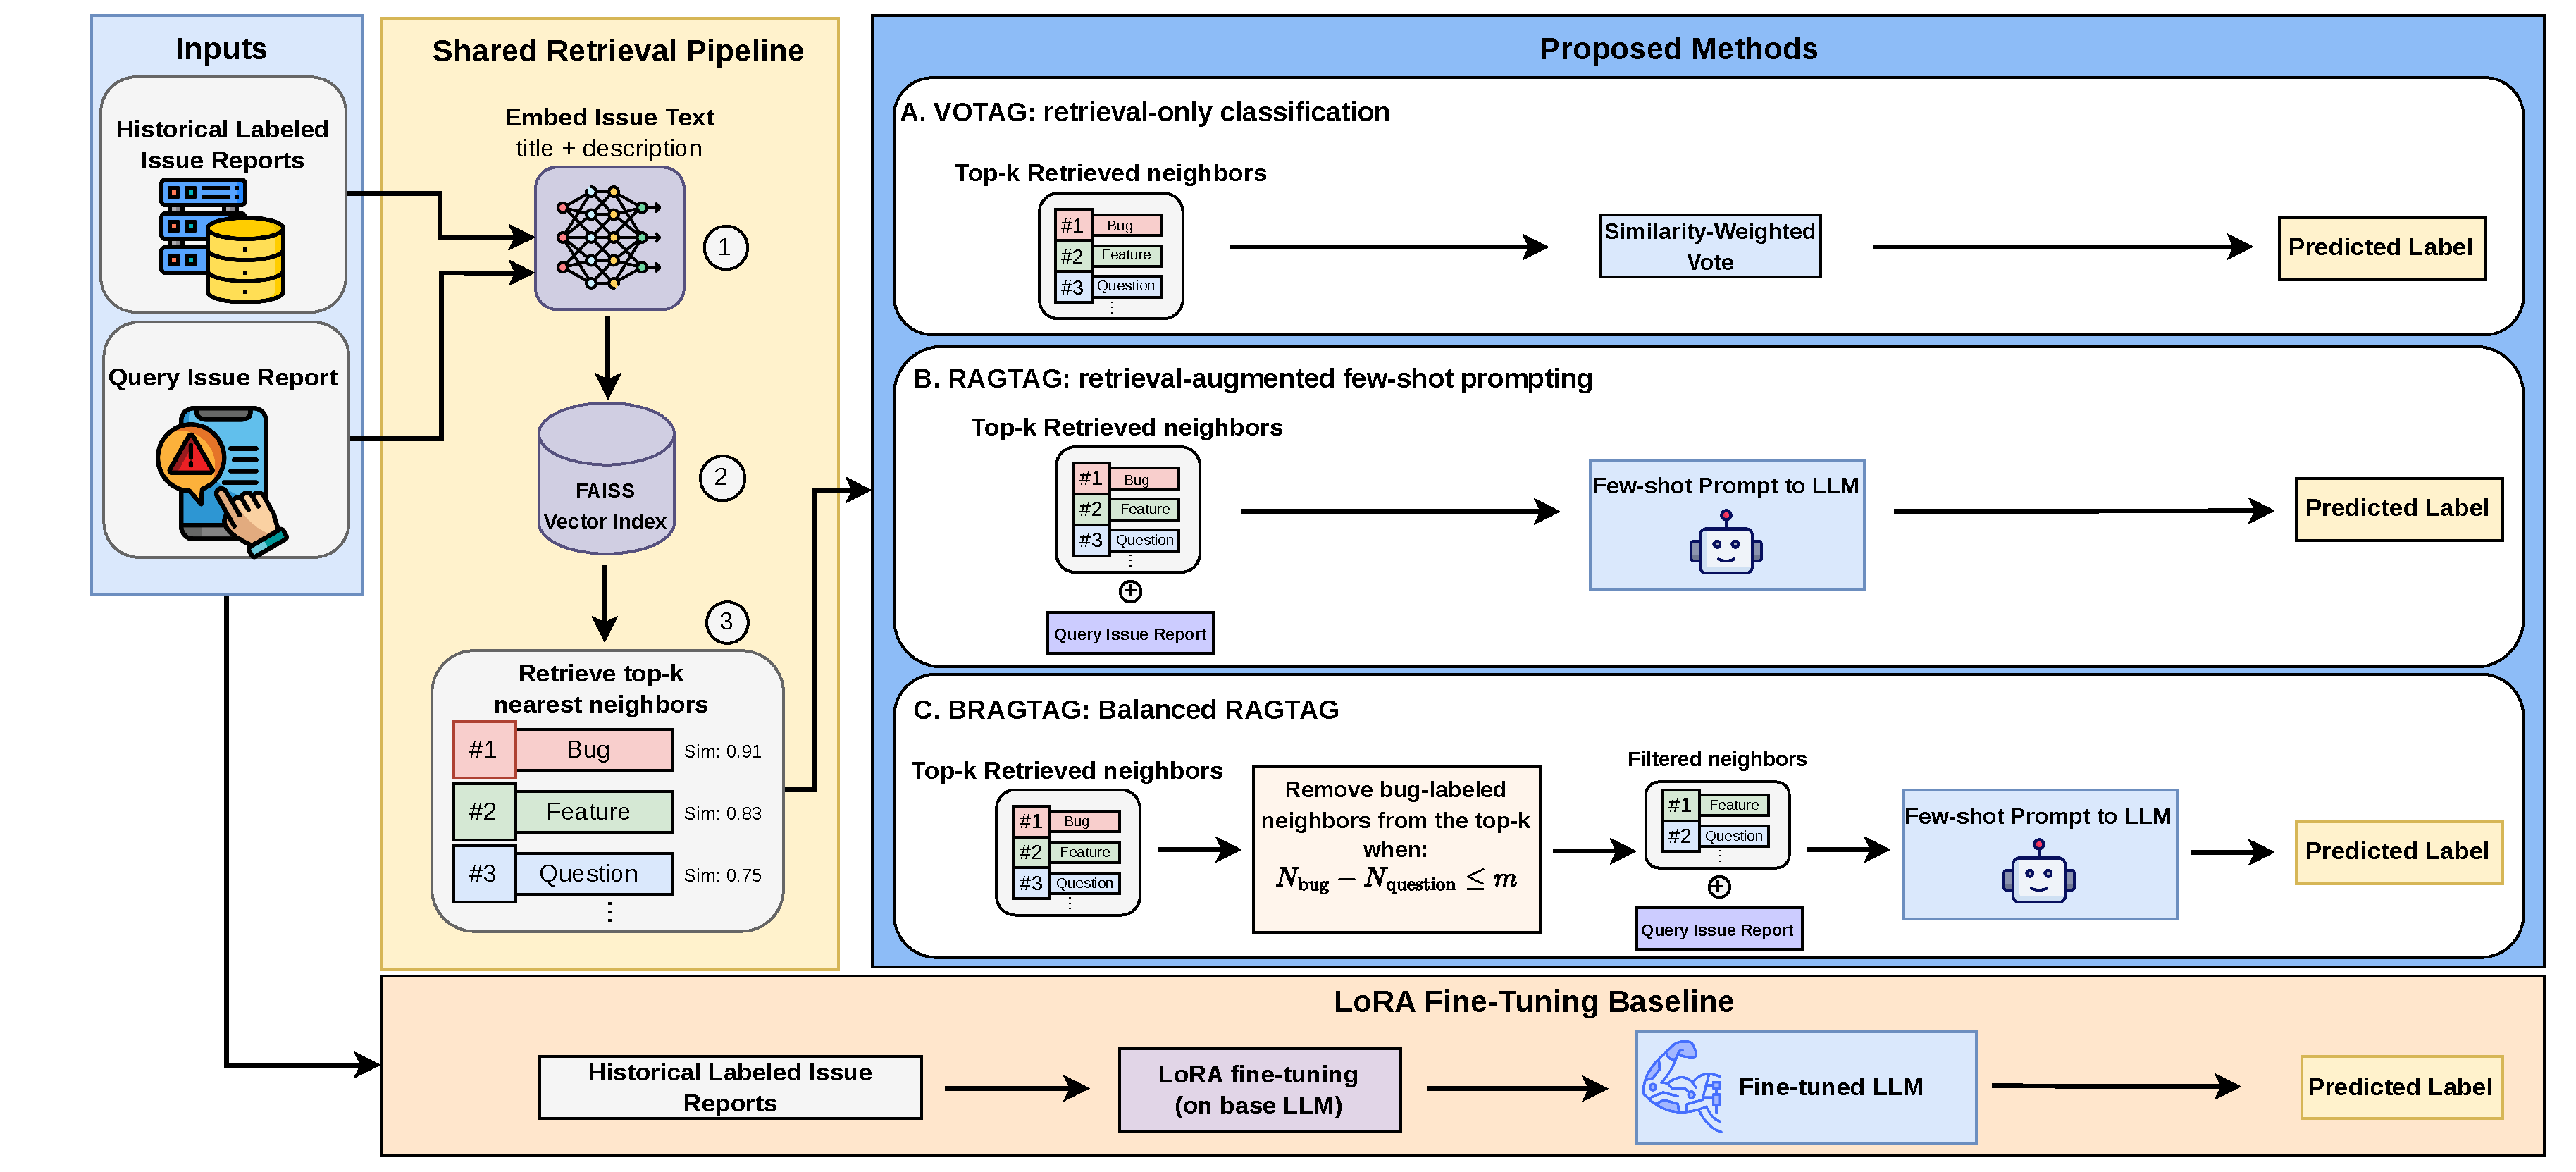
\includegraphics[width=0.88\textwidth]{figures/fao.pdf}
    \caption{Overview of the $k$NN voting baseline, retrieval-augmented few-shot prompting (RAG), filtered RAG, and the LoRA fine-tuning baseline.}
    \label{fig:approach-overview}
\end{figure*}

All retrieval-based classifiers share one retrieval step (\cref{sec:retrieval}). The \knn\ baseline labels the query from its neighbors' labels alone, \rag\ shows the neighbors to the LLM as labeled examples, and \frag\ removes bug-labeled examples for suspected questions. We compare the two RAG variants with LoRA fine-tuning of the same LLMs (\cref{sec:finetune}); \cref{fig:approach-overview} shows all four approaches.

\subsection{Problem Formulation}
\label{sec:problem}
Given a query issue report, we classify it into only one of the three labels: \emph{bug}, \emph{feature}, or \emph{question}. Only the issue's title and description text are used for classification with no other signals from the issue tracker. The defined label space is adopted directly from prior IRC studies~\cite{aracena2024applyinglargelanguagemodels,aracena2025applying,izadi2022catiss,kallis2019ticket,antoniol2008bug}. 

\subsection{Indexing and Retrieval}
\label{sec:retrieval}
To prepare the issues for retrieval based on textual similarity, we first embed their textual content (i.e., \textit{title} + \textit{description}). We do not embed the issue labels. Instead, we retain them as metadata associated with each embedded issue. To generate the embeddings, we use the \texttt{all-MiniLM-L6-v2} model from the Sentence-Transformers library~\cite{reimers2019sentence}. We selected this model due to its lightweight architecture, fast performance, and effectiveness on issue report text~\cite{huang2025back}. The embeddings are then indexed using the FAISS vector database library~\cite{douze2025faiss}, which provides efficient high-dimensional similarity retrieval. At the retrieval stage, the query issue is first embedded with the same model. Next, FAISS calculates the cosine similarity of indexed issue reports to the query, and returns the top-$k$ nearest neighbors, ordered by descending similarity.

%%%%%%%%%%%%%%%%%%%%
\subsection{$k$NN Voting Baseline}
\label{sec:approach-votag}
The \knn baseline labels the query by a similarity-weighted vote over the labels of its top-$k$ neighbors, following the distance-weighted $k$-nearest-neighbor rule~\cite{cover1967nearest, dudani1976distance}.\footnote{Squared-similarity weighting and uniform majority were also evaluated, but were outperformed by similarity-weighted voting.} Because it uses no LLM, \knn\ measures how much label information the neighbors carry. Its peak sets the largest $k$ we give the LLM (\cref{sec:rq1}), and it labels invalid LLM outputs in the fallback (\cref{sec:rq3}). Formally, for a
query issue $q$ with retrieved neighbors $\{(n_i, l_i, s_i)\}_{i=1}^{k}$, where
$n_i$ is the $i$-th nearest neighbor with label $l_i$ and cosine similarity $s_i$ to $q$, the predicted label $\hat{y}$ is given by:

\begin{equation}
    \hat{y} = \operatorname*{arg\,max}_{c \in \mathcal{L}}
    \sum_{i=1}^{k} s_i \cdot \mathbf{1}[l_i = c],
    \label{eq:votag}
\end{equation}

where $\mathcal{L}$ is the label set, and $\mathbf{1}[l_i = c]$ is the indicator function that equals $1$ when neighbor $i$ has label $c$ and $0$ otherwise. For each label, \knn\ sums the cosine similarities of the neighbors that carry that label, and the $\operatorname*{arg\,max}$ operator returns the label with the largest total sum. It breaks ties by returning the label of the most similar neighbor in the tied classes.



%%%%%%%%%%%%%%%%%%%%%%%%%%%%%%%%
\begin{comment} %% Prompt box with title bar
\definecolor{prompttitlebar}{HTML}{3A3A55}
\definecolor{promptbody}{HTML}{F2F2FF}
\begin{figure}[t]
    \centering
    \begin{tikzpicture}[
        font=\fontsize{6}{7}\selectfont\ttfamily,
        sec/.style={anchor=north, text width=10.3cm, align=left,
                    inner xsep=0.2cm, inner ysep=6pt, fill=promptbody},
        seclabel/.style={anchor=east, font=\sffamily\scriptsize,
                    align=right, text=prompttitlebar},
    ]
    % --- title bar ---
    \node[anchor=north, text width=10.3cm, align=center,
          inner xsep=0.2cm, inner ysep=4pt, fill=prompttitlebar,
          text=white, font=\sffamily\small\bfseries] (title) at (0,0)
        {Retrieval-augmented few-shot prompt format};
    % --- (1) system message ---
    \node[sec, below=0pt of title.south] (s1)
        {Classify the GitHub issue into exactly one category: bug, feature,
         or question. Respond with ONLY the label wrapped in XML tags
         (e.g., <label>bug</label>). Do NOT write anything else --- no
         explanation, no reasoning, no extra text.};
    % --- (2) retrieved examples ---
    \node[sec, below=0pt of s1.south] (s2)
        {Here are some examples of correctly classified issues:\\[2pt]
         -{}-{}- Example 1 -{}-{}-\quad Title: \textit{$\langle$title$\rangle$}\quad
         Body: \textit{$\langle$body$\rangle$}\quad
         Answer: <label>feature</label>\\[2pt]
         \textit{$\cdots$}\\[2pt]
         -{}-{}- Example K -{}-{}-\quad Title: \textit{$\langle$title$\rangle$}\quad
         Body: \textit{$\langle$body$\rangle$}\quad
         Answer: <label>bug</label>};
    % --- (3) query issue ---
    \node[sec, below=0pt of s2.south] (s3)
        {Now, classify the following target issue:\quad
         Title: \textit{$\langle$query title$\rangle$}\quad
         Body: \textit{$\langle$query description$\rangle$}};
    % --- dashed section dividers, extended beyond the border ---
    \draw[dashed] ([xshift=-1.9cm]s1.south west) -- ([xshift=0.35cm]s1.south east);
    \draw[dashed] ([xshift=-1.9cm]s2.south west) -- ([xshift=0.35cm]s2.south east);
    % --- outer border ---
    \draw[line width=0.8pt] (title.north west) rectangle (s3.south east);
    % --- section names, outside the border on the left ---
    \node[seclabel] at ([xshift=-0.22cm]s1.west) {System message};
    \node[seclabel] at ([xshift=-0.22cm]s2.west) {Retrieved examples\\($K$ nearest neighbors)};
    \node[seclabel] at ([xshift=-0.22cm]s3.west) {Query issue};
    \end{tikzpicture}
    \caption{The retrieval-augmented few-shot prompt structure used for \rag and
    \frag.}
    \label{fig:prompt}
\end{figure}
\end{comment}
%%%%%%%%%%%%%%%%%%%%%%%%%%%%%%%%

\definecolor{prompttitlebar}{HTML}{3A3A55}
\definecolor{promptbody}{HTML}{F2F2FF}

% Column-width prompt figure. Geometry: a 1.85cm label gutter on the left and a
% 0.10cm divider overhang on the right, so the drawing is exactly \columnwidth.
\begin{figure}[t]
    \centering
    \begin{tikzpicture}[
        font=\fontsize{6}{7}\selectfont\ttfamily,
        sec/.style={anchor=north, align=left,
                    text width=\dimexpr\columnwidth-2.0cm-0.4cm\relax,
                    inner xsep=0.2cm, inner ysep=5pt, fill=promptbody},
        seclabel/.style={anchor=east, font=\sffamily\scriptsize,
                    align=right, text=prompttitlebar, text width=1.55cm,
                    inner sep=0pt},
    ]

    % --- (1) system message ---
    \node[sec] (s1) at (0,0)
        {Classify the GitHub issue into exactly one category: bug, feature,
         or question. Respond with ONLY the label wrapped in XML tags
         (e.g., <label>bug</label>). Do NOT write anything else --- no
         explanation, no reasoning, no extra text.};

    % --- (2) retrieved examples ---
    \node[sec, below=0pt of s1.south] (s2)
        {Here are some examples of correctly classified issues:\\[2pt]
         -{}-{}- Example 1 -{}-{}-\quad Title: \textit{$\langle$title$\rangle$}\quad
         Body: \textit{$\langle$body$\rangle$}\quad
         Answer: <label>feature</label>\\[2pt]
         \textit{$\cdots$}\\[2pt]
         -{}-{}- Example $k$ -{}-{}-\quad Title: \textit{$\langle$title$\rangle$}\quad
         Body: \textit{$\langle$body$\rangle$}\quad
         Answer: <label>bug</label>};

    % --- (3) query issue ---
    \node[sec, below=0pt of s2.south] (s3)
        {Now, classify the following target issue:\quad
         Title: \textit{$\langle$query title$\rangle$}\quad
         Body: \textit{$\langle$query description$\rangle$}};

    % --- dashed section dividers, extended into the label gutter ---
    \draw[dashed] ([xshift=-1.85cm]s1.south west) -- ([xshift=0.10cm]s1.south east);
    \draw[dashed] ([xshift=-1.85cm]s2.south west) -- ([xshift=0.10cm]s2.south east);

    % --- outer border ---
    \draw[line width=0.8pt] (s1.north west) rectangle (s3.south east);

    % --- section names, in the gutter on the left ---
    \node[seclabel] at ([xshift=-0.15cm]s1.west) {System\\message};
    \node[seclabel] at ([xshift=-0.15cm]s2.west) {Retrieved\\examples\\($k$ nearest\\neighbors)};
    \node[seclabel] at ([xshift=-0.15cm]s3.west) {Query\\issue};

    \end{tikzpicture}
    \caption{The retrieval-augmented few-shot prompt structure used for \rag\ and
    \frag.}
    \label{fig:prompt}
\end{figure}
%%%%%%%%%%%%%%%%%%%%%%%%%%%%%%%%

\subsection{Retrieval-Augmented Few-Shot Prompting (RAG)}
\label{sec:approach-ragtag}
\rag shows the query's top-$k$ neighbors (\cref{sec:retrieval}) to the LLM as labeled examples. We use the neighbors, rather than randomly chosen labeled issues, because similar examples can outperform random ones~\cite{liu2022makes, yu2023retrieval} and because the neighbors' labels alone reach 59.5\% macro $F_1$ (\cref{sec:rq1}).
We create the few-shot prompt in three parts as shown in \figref{prompt}. First, the system message frames the classification task and the label space. Second, the top-$k$ nearest neighbors are listed in retrieval order (descending similarity), each formatted as \textit{title + description + label}. Finally, the query issue closes the prompt, since LLMs use information at the end of a long context better than in its middle~\cite{liu2024lost}. With $k{=}0$, the prompt has no examples and \rag\ becomes zero-shot prompting, as in prior work~\cite{colavito2025benchmarking}.

We evaluate $k \in \{0, 1, 3, 6, 9, 12, 15\}$, up to \knn's peaks at $k{=}15$--16 (\cref{sec:rq1}). The maximum prompt sequence length is set to 8,192 tokens.\footnote{Maximum prompt sequence length is selected empirically. 8,192 tokens offered the best trade-off between macro $F_1$ and inference speed across our preliminary experiments.} Roughly 30\% of the context quota is reserved for the query issue and 70\% for the neighbors. If the neighbors exceed their overall quota, they are truncated proportionally based on their length (longer neighbors get more truncation). The query issue gets truncated if it exceeds its budget as well. Truncation happens on the right side of the
description text, preserving all titles and labels (if any).
The LLM is instructed to generate the predicted label wrapped in XML tags (e.g. \texttt{<label>bug</label>}). The labels of the presented examples also follow the same format. We use a regular expression to extract the predicted label. Outputs that contain none of the three labels are marked as \textit{invalid}. Finally, models are loaded with Unsloth\footnote{\url{https://unsloth.ai}} for memory efficiency, and the temperature is set at 0.1 for deterministic classifications.
%%%%%%%%%%%%%%%%%%%%%
\subsection{Filtered RAG}
\label{sec:approach-bragtag}
\rag's most frequent error is labeling questions as bugs (\cref{sec:rq1}), a known weakness of \irc\ methods~\cite{colavito2024impact, colavito2025benchmarking}. The models make this error even at zero-shot, so we hypothesize that bug-labeled examples retrieved for a question reinforce it. \Frag\ therefore removes the bug-labeled examples from the prompt when the neighbors suggest that the query is a question, that is, when $N_\text{bug} - N_\text{question} \le m$, where $N_\text{label}$ is the number of neighbors with that label among the top $k$ and $m$ is a small positive margin. For example, with $k{=}12$ and $m{=}3$, a query whose neighbors are six bugs, four questions, and two features has $N_\text{bug} - N_\text{question} = 2$, so the six bug examples are removed and the prompt shows the remaining six.

We calibrated $m$ before testing, on a validation split of the labeled issues. From each project's 300 labeled issues, 30 issues stratified by label serve as queries and the other 270 as the retrieval index, mirroring the project-specific setting (\cref{sec:setup-dataset}). On this split, true questions retrieve nearly balanced bug and question neighbors, with on average 1.36 more question than bug neighbors over $k\in[1,15]$. We swept $m\in\{1,\dots,5\}$, where 5 is the 95th percentile of $N_\text{bug} - N_\text{question}$ for true questions, and chose $m{=}3$ as the best trade-off between firing for questions and for bugs. Averaged over $k$, it fires for 89.1\% of true questions and 56.7\% of true bugs. Otherwise, \frag\ is identical to \rag.

\subsection{LoRA Fine-Tuning Baseline}
\label{sec:finetune}
Prior LLM-based \irc\ studies fine-tune open LLMs on labeled issue reports with LoRA~\cite{hu2022lora, heo2025study, aracena2025applying}. Each training example is an instruction prompt with the issue's title and description as input and its label as output. We adopt the prompt template of these studies~\cite{heo2025study,aracena2025applying} verbatim, so that our baseline reproduces their method. At inference, the fine-tuned model receives the query issue in the same format and completes the empty label field. A regular expression extracts the label, and outputs that contain none of the three labels are \textit{invalid}.

Training hyperparameters follow prior work~\cite{heo2025study,aracena2025applying}. The LoRA rank and alpha are set to 16, with a learning rate of $2 \times 10^{-4}$ and the paged AdamW 8-bit optimizer. Training runs for 3 epochs with a per-device batch size of 1 and gradient accumulation steps of 16. The maximum prompt sequence length is 2,048 tokens, which leaves 94.9\% of the test issues untruncated; longer issues are truncated from the right of their description.
Similar to \rag and \frag, the models are loaded with Unsloth and the temperature is set at 0.1.
